% !TeX spellcheck = en_EN-English

\chapter{Proposed method}

Task of predicting future cost of a patient can be split input multiple sub-tasks which follow each other. The sub-tasks are these:

\begin{enumerate}
	\item Embed patient history into numerical vectors
	\item Compute expected number of records patient would have in next year
	\item Predict future records for patient
	\item Predict cost of each future record
	\item Complete total cost of patient for next year
\end{enumerate}


% !TeX spellcheck = en_EN-English

\section{Embedding of Patient}
\label{embedding}

The first sub-task in predicting a patient’s future costs is to embed each patient record into a numerical vector that can be interpreted by a neural network. Our main goal was to create embeddings that retain similarity information-meaning that records with similar diagnoses, drugs, and medical procedures receive similar embeddings. We define similarity using the Euclidean distance between embedding vectors. Preserving similarity is important because it simplifies the prediction task: the model only needs to predict a closely related record, rather than the exact one.
\\

For each patient record, we embed four distinct attributes. The first, and simplest to implement, is the timestamp, which is calculated using numerical and date values. The remaining three attributes, which are diagnosis, medical procedure, and prescribed drug, are more complex to embed.

\subsection{Timestamp}

The attribute we refer to as the timestamp of a patient’s record can be more precisely described as an approximation of the patient’s age at the time of either a medical procedure or drug prescription. This timestamp is calculated using two available pieces of information: the patient’s age in years and the date of the record. The specific procedures we use to compute this timestamp are detailed in section \ref{timespampImple}. In general, we identify the first record, compute its timestamp based on the patient’s age as an approximate age in days at that point, and then calculate each subsequent timestamp as the timestamp of the first record plus the difference in record dates. In this way, each timestamp provides an approximation of the patient’s age while also conveying the order of records and the relative timeframe between any two records.

\subsection{Diagnosis embedding}
\label{diagEmb}

The base diagnosis information we embedded was the ICD-10-CM code for the disease. ICD-10-CM stands for "International Classification of Diseases, Tenth Revision, Clinical Modification," which is used to code and classify medical diagnoses \cite{cdcICD10CM}. In Slovakia, this classification system is known as MKCH-10-SK (Medzinárodná klasifikácia chorôb) \cite{ncziMKCH}.
\\

\begin{figure}[!h]
	\centering
	
	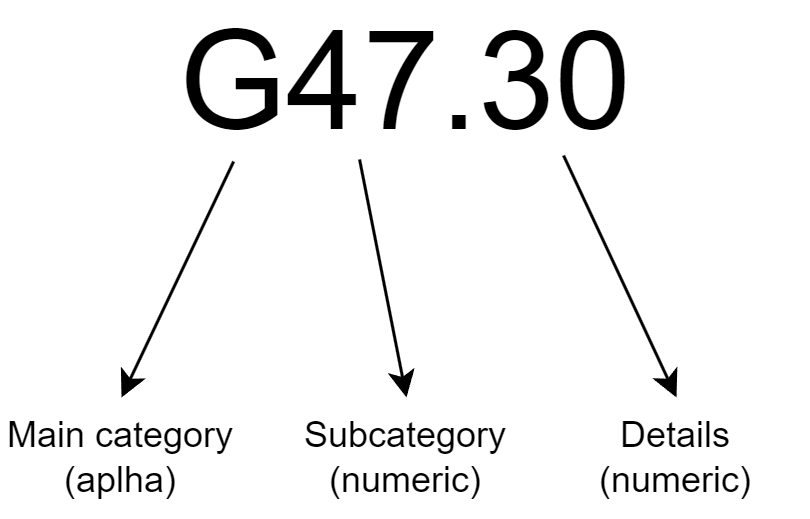
\includegraphics[width=0.8\textwidth]{images/ICD-10-CM.png}
	
	\caption{Structure of MKCH-10 code.}
	\label{fig:icd-10-cm}
\end{figure}

This code consists of three parts, as shown in Fig. \ref{fig:icd-10-cm}. The first part is a letter that encodes the main categories of diseases, also known as chapters. For example, codes starting with G represent diseases of the nervous system. Following this, there are two numeric characters that further specify the subcategory of the disease, such as codes from G40 to G47, which are episodic and paroxysmal disorders, with G47 specifically being sleep disorders. We observe that episodic and paroxysmal disorders only extend up to G47, meaning that theoretically, subgroups G48 and G49 could exist with a 4 in the second position but would not belong to the same G4 subcategory as G40 or G47 \label{mkch_subdiv}. Fortunately, this is not the case; when a higher-level subcategory (like G4) does not have 10 lower-level subcategories (like G47), these subcategories do not exist at all. If there are more than 10 lower-level subcategories, they are assigned multiple consecutive higher-level subcategories, such as disorders of other endocrine glands, which span from E20 to E35. The code then contains a dot, after which there are characters that further describe the details of the disease, such as etiology, anatomic site, and severity. According to the official documentation, ICD-10-CM codes can be up to 7 characters long, meaning that after the first three characters specifying the category, there can be up to 4 additional alphanumeric characters to further specify the disease \cite{icd10expl}. However, the version used in Slovak healthcare database, MKCH-10, contains only up to two numeric characters to specify the disease \cite{mkch10expl}. These details are organized such that the first position conveys higher-level information than the second; for example, G47.3 is sleep apnea, and G47.30 is primary central sleep apnea.
\\

To embed this code, we first split it into its three parts and separately embed each part. We then concatenated the embeddings of each part to obtain the final disease embedding. For the main category, we generated random vectors from a uniform distribution for each letter in the English alphabet (representing all main categories). We chose random vectors to ensure relatively similar distances between any two main categories, as there are no inherent relationships among these categories. We also considered using one-hot encoding, which would make the distance between every pair of categories identical, but opted against it because this approach would constrain the vector length.
\\

In embedding the second part, which is the subcategory, we used a different approach. For each number between 00 and 99 (all possible values of this part), we assigned a linearly spaced number within a chosen interval. This value was then repeated multiple times to create a vector. This repetition was implemented to encode the importance of this part of the code. This approach has both advantages and disadvantages. The advantage is that we can be sure that closely related disease subgroups, like G46 and G47, would receive similar embeddings since their subgroup codes are close on the number line. However, there are also two disadvantages. The first is that G49 and G50 would be similarly close as G46 and G47, but fortunately, in most cases, either the X9 code does not exist at all, creating a gap, or if the X9 code exists it belongs to a category that goes past X as a higher-level subgroup. Another disadvantage is that the distance between two higher-level subgroups can vary quite dramatically, even though in reality there might not be a reason for such a difference. For example, using this approach, the higher-level subgroup G40–G47 is much closer to subgroup G50–G59 than to G80–G83.
\\

Finally, to embed details, we used the same approach as for subgroups, since these codes function similarly. The only difference was that not all codes included second-level details. In such cases, we added "5" as a proxy value to minimize the average distance from all potential codes sharing the same first-level detail code (with second-level information) while maximizing the average distance to codes with different first-level details.
\\

Once all parts were embedded, we created the final embedding by concatenating them. To encode the importance of each part, we assigned different vector lengths. This works because each value in the vector has the same mean and variance. We encoded the importance hierarchically: the main category received the longest embedding, subgroups a medium length, and details the shortest embedding.

\subsection{Drug embedding}
\label{drugEmb}

Similarly to diagnosis, to embed drug information we used the international code associated with each drug. In the case of drugs, this was the Anatomical Therapeutic Chemical (ATC) classification system. Like the MKCH-10 code, the ATC code can be split into multiple parts, with each subsequent part providing more detailed information. The ATC code consists of five parts or levels.
\\

Structure of the ATC code:

\begin{itemize}
	\item First level: A single letter representing one of 14 main anatomical or pharmacological groups (e.g., "C" for cardiovascular system). These groups are shown in Fig. \ref{fig:atc_l1}.
	\item Second level: A two-digit number specifying a pharmacological or therapeutic subgroup (e.g., "C03" for diuretics).
	\item Third and fourth levels: Each uses a single letter to further classify pharmacological, therapeutic, or chemical subgroups (e.g., "C03C" for high-ceiling diuretics and "C03CA" for sulfonamide derivatives).
	\item Fifth level: A two-digit number identifying the specific chemical substance (e.g., "C03CA01" for furosemide).
\end{itemize}

\begin{figure}[!h]
	\centering
	
	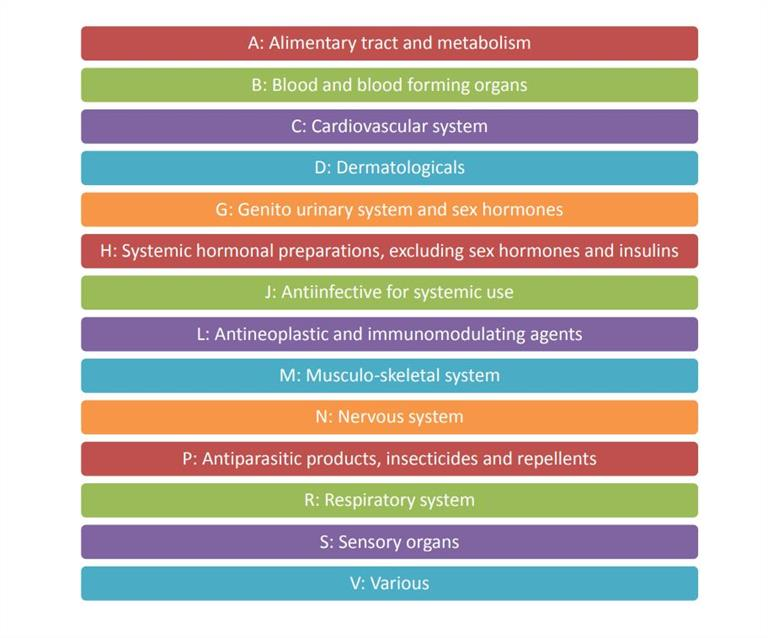
\includegraphics[width=0.8\textwidth]{images/atc_l1_classification_who.jpg}
	
	\caption{Fourteen main anatomical or pharmacological groups and their corresponding first level ATC code \cite{atc_who}.}
	\label{fig:atc_l1}
\end{figure}

Embedding was performed in a manner very similar to the diagnosis embedding: each level was embedded separately, and the final embedding was created by concatenating them. In this case, each level was embedded using a random vector drawn from a uniform distribution. We chose random vectors because none of the ATC levels contain internal subgroupings analogous to the hierarchical subgroups seen in diagnosis codes (see \ref{mkch_subdiv} for subgroup code details). To encode the importance of each level, we again varied the lengths of the random vectors. This approach ensures that the similarity between codes depends more on matches in the lower, more important levels than in the higher ones.
\\

\subsection{Medical procedure embedding}
\label{procedureEmb}

The final component to embed was medical procedures. In this case, no structured code is implemented within the Slovak healthcare system. To address this, we embedded textual descriptions of procedures using two approaches:

\begin{itemize}
	\item Multilingual Large Language Model (LLM): We selected the LaBSE model (section \ref{theoryLaBSE}), trained on multiple languages including Slovak. LaBSE generates similar embeddings for semantically equivalent sentences across languages, which aligns with medical terminology often being international.
	\item Slovak-specific Word2Vec: A Word2Vec model (section \ref{theoryW2v}) trained exclusively on Slovak textual data.
\end{itemize}

For both methods, we reduced the dimensionality of the resulting embeddings using Principal Component Analysis (PCA) to eliminate low-variance dimensions encoding minimal information.
\\

To construct the final record embedding, we concatenated all four components (timestamp, diagnosis, medical procedure, and prescribed drug). Since timestamp and diagnosis are always available, we substituted missing drug or procedure data with zero vectors of matching length. This neutral substitution preserves compatibility between datasets while maintaining centered embeddings.

\section{Prediction of future number of records}

Our task is to get information about how much will cost patient in the future, more specifically, how much it will cost in the next. Since our approach predicts future records, assign to them cost and sum the cost into resulting cost, we need to somehow be able to assess how many records need to be generated in order to simulate approximately next year. For this task we tried two different approaches.
\\

First approach was to predict approximate number of records using linear regression which gets counts of records from previous years and predict next one. Other approach used stopping criterion, which uses timestamp information which is available in each input and generated records, and stop generating once difference between last timestamp from patient data and last generated timestamp surpass one year threshold.
\\

Each of these method have it's own disadvantages. In case of linear regression, number of records per year can vary significantly, so even though we expect increase \cite{num_of_vis} regression might not be able to catch this trend, especially if patient data consist of only few years in the past. Potential issue with second approach is that it's dependent on how well model learned that timestamp should always increase.  

% !TeX spellcheck = en_EN-English

\section{Future record prediction}
\label{record_prediction}

%This task is both the most important and the most challenging to train. Our goal is to develop a model capable of predicting a patient's potential next record based on their previous ones. Generally, this task is nearly impossible with the amount of information available, as numerous factors influence whether, when, and what new disease a patient might contract, how their current state will evolve, and what specific actions a doctor will take.
%\\

This task is both the most important and the most challenging to train. Our goal is to develop a model capable of predicting a patient’s potential next record based on their previous ones. In general, this is nearly impossible given the available information, as many other factors influence if, when, and what new disease a patient might contract, how their condition will evolve, and what actions a doctor will take.
\\

Fortunately, our ultimate goal is not to predict a patient's specific future but to estimate the likely total cost of their future records. We anticipate that even if we cannot predict exact outcomes, we can still estimate the overall cost.
\\

To achieve this prediction, we experimented with multiple models. The first three models we tested were Recurrent Neural Networks (RNNs): multi-layer Elman RNN, multi-layer Gated Recurrent Unit (GRU) RNN, and multi-layer Long Short-Term Memory (LSTM) RNN. The architecture of these models is detailed in Sec. \ref{theoryRNN}. The last model we tried was a Transformer, specifically a Decoder-only Transformer model, explained in Sec. \ref{theoryTrans}.



% !TeX spellcheck = en_EN-English

\section{Record cost prediction}
\label{recCostPred}

The next step in total cost prediction involves estimating the cost of individual records. This is necessary because the future records we predict lack cost information, requiring an additional model to determine it. We adopted this approach to leverage the entire record for prediction, rather than relying solely on a single cost dimension that could have been added. For this task, we selected a standard Multilayer Perceptron (MLP), a multi-layered, fully-connected feed-forward neural network, whose architecture is detailed in Sec. \ref{MLP}.
\\

We also trained a Gradient Boosting model and a Ridge regression model for comparative analysis. These were chosen to represent two distinct model families: decision trees (Gradient Boosting) and linear regression (Ridge). We selected these specific representatives because they employ more sophisticated techniques than base models in their respective groups and have demonstrated performance comparable to, if not better than, artificial neural networks in similar studies, such as the work by Mohammad Amin Morid et al. \cite{morid2018supervised} (discussed in Chap. \ref{simStudy}).